%% Lab Report for EEET2493_labreport_template.tex
%% V1.0
%% 2019/01/16
%% This is the template for a Lab report following an IEEE paper. Modified by Francisco Tovar after Michael Sheel original document.


%% This is a skeleton file demonstrating the use of IEEEtran.cls
%% (requires IEEEtran.cls version 1.8b or later) with an IEEE
%% journal paper.
%%
%% Support sites:
%% http://www.michaelshell.org/tex/ieeetran/
%% http://www.ctan.org/pkg/ieeetran
%% and
%% http://www.ieee.org/

%%*************************************************************************
%% Legal Notice:
%% This code is offered as-is without any warranty either expressed or
%% implied; without even the implied warranty of MERCHANTABILITY or
%% FITNESS FOR A PARTICULAR PURPOSE! 
%% User assumes all risk.
%% In no event shall the IEEE or any contributor to this code be liable for
%% any damages or losses, including, but not limited to, incidental,
%% consequential, or any other damages, resulting from the use or misuse
%% of any information contained here.
%%
%% All comments are the opinions of their respective authors and are not
%% necessarily endorsed by the IEEE.
%%
%% This work is distributed under the LaTeX Project Public License (LPPL)
%% ( http://www.latex-project.org/ ) version 1.3, and may be freely used,
%% distributed and modified. A copy of the LPPL, version 1.3, is included
%% in the base LaTeX documentation of all distributions of LaTeX released
%% 2003/12/01 or later.
%% Retain all contribution notices and credits.
%% ** Modified files should be clearly indicated as such, including  **
%% ** renaming them and changing author support contact information. **
%%*************************************************************************

\documentclass[journal]{IEEEtran}

% *** CITATION PACKAGES ***
\usepackage[style=ieee]{biblatex} 

% *** MATH PACKAGES ***
\usepackage{amsmath}

% *** PDF, URL AND HYPERLINK PACKAGES ***
\usepackage{url}
% correct bad hyphenation here
\hyphenation{op-tical net-works semi-conduc-tor}
\usepackage{graphicx}  %needed to include png, eps figures
\usepackage{float}  % used to fix location of images i.e.\begin{figure}[H]

%https://tex.stackexchange.com/questions/230828/when-referencing-a-figure-make-text-and-figure-name-clickable
\usepackage[colorlinks]{hyperref}

\usepackage{pdflscape}
\usepackage{multicol}
\usepackage{listings}
\usepackage{color}
\usepackage[dvipsnames]{xcolor}

\definecolor{dkgreen}{rgb}{0,0.6,0}
\definecolor{gray}{rgb}{0.5,0.5,0.5}
\definecolor{mauve}{rgb}{0.58,0,0.82}

\lstset{frame=tb,
  language=C++,
  aboveskip=3mm,
  belowskip=3mm,
  showstringspaces=false,
  columns=flexible,
  basicstyle={\small\ttfamily},
  numbers=none,
  numberstyle=\tiny\color{gray},
  keywordstyle=\color{blue},
  commentstyle=\color{dkgreen},
  stringstyle=\color{mauve},
  breaklines=true,
  breakatwhitespace=true,
  tabsize=3
}

\lstdefinelanguage{Ini}
{
    basicstyle=\ttfamily\small,
    columns=fullflexible,
    morecomment=[s][\color{mauve}\bfseries]{[}{]},
    morecomment=[l]{\#},
    morecomment=[l]{;},
    commentstyle=\color{gray}\ttfamily,
    morekeywords={},
    otherkeywords={=,:},
    keywordstyle={\color{green}\bfseries}
}

% https://github.com/GothenburgBitFactory/guides/blob/master/20151107_de_openrheinruhr/yaml_syntax_highlighting.tex
%%%%%%%%%%%%%%%%%%%%%%%%%%%%%%%%%%%%%%%%%%%%%%%%%%%%%%
%%%%%%%%%%% YAML syntax highlighting %%%%%%%%%%%%%%%%%

% http://tex.stackexchange.com/questions/152829/how-can-i-highlight-yaml-code-in-a-pretty-way-with-listings

% here is a macro expanding to the name of the language
% (handy if you decide to change it further down the road)
\newcommand\YAMLcolonstyle{\color{red}\mdseries}
\newcommand\YAMLkeystyle{\color{black}\bfseries}
\newcommand\YAMLvaluestyle{\color{blue}\mdseries}

\makeatletter

\newcommand\language@yaml{yaml}

\expandafter\expandafter\expandafter\lstdefinelanguage
\expandafter{\language@yaml}
{
  keywords={true,false,null,y,n},
  keywordstyle=\color{darkgray}\bfseries,
  basicstyle=\YAMLkeystyle,                                 % assuming a key comes first
  sensitive=false,
  comment=[l]{\#},
  morecomment=[s]{/*}{*/},
  commentstyle=\color{purple}\ttfamily,
  stringstyle=\YAMLvaluestyle\ttfamily,
  moredelim=[l][\color{orange}]{\&},
  moredelim=[l][\color{magenta}]{*},
  moredelim=**[il][\YAMLcolonstyle{:}\YAMLvaluestyle]{:},   % switch to value style at :
  morestring=[b]',
  morestring=[b]",
  literate =    {---}{{\ProcessThreeDashes}}3
                {>}{{\textcolor{red}\textgreater}}1     
                {|}{{\textcolor{red}\textbar}}1 
                {\ -\ }{{\mdseries\ -\ }}3,
}

% switch to key style at EOL
\lst@AddToHook{EveryLine}{\ifx\lst@language\language@yaml\YAMLkeystyle\fi}
\makeatother

\newcommand\ProcessThreeDashes{\llap{\color{cyan}\mdseries-{-}-}}

%%%%%%%%%%% YAML syntax highlighting %%%%%%%%%%%%%%%%%
%%%%%%%%%%%%%%%%%%%%%%%%%%%%%%%%%%%%%%%%%%%%%%%%%%%%%%

\begin{document}

% paper title
\title{Arduino Lab 1}

% author names 
\author{Knut Ola Nøsen,
    Kristian Hansen,
}% <-this % stops a space

% The report headers
\markboth{IELET1002 DATATEKNIKK. LAB. REPORT 1, JANUARY 2022}%do not delete next lines
{Shell \MakeLowercase{\textit{et al.}}: Bare Demo of IEEEtran.cls for IEEE Journals}

% make the title area
\maketitle

% As a general rule, do not put math, special symbols or citations
% in the abstract or keywords.
\begin{abstract}
    The project centers around an ultrasonic proximity sensor, and an OLED Display that shows a revolving set of sensor readings in real-time.
    The purpose of this project is to demonstrate a situation where many isolated components can function in conjunction, while still not interfearing with each others operation.
    Furthermore, the project explores the use of Software-Libraries to improve the quality of the final product, while reducing TTC (Time To Completion).
    The contents of this paper reflects the aspects most in focus during the execution of the lab. That being my research into best-practices
    in the IoT industry, rather than the project itself.
\end{abstract}

\begin{IEEEkeywords}
    Arduino, OLED, C++, PlatformIO, Code-Library, Header File, Test Driven Development, Unit Test, ASSERT, HE-SR04
\end{IEEEkeywords}

\section{Theory}
% Here we have the typical use of a "W" for an initial drop letter
% and "RITE" in caps to complete the first word.
% You must have at least 2 lines in the paragraph with the drop letter
% (should never be an issue)

\IEEEPARstart{T}{he} HE-SR04 ultrasonic sensor is a low-cost Arduino component for measuring short distances. It gives a relatively inaccurate reading, and out of the box is subject to signal noise. For this reason, a Median-Filter has been implemented through software, to remove the more extreme spikes in telemetry. The inner workings of the ultrasonic sensor are based on ultrasound, commonly found in animals like bats and whales. The following code shows a crude implementation of this sensor:
\begin{lstlisting}
float getDistance(int trigger, int echo) {
    // Disable speaker
    digitalWrite(trigger, LOW);
    // Wait until any existing sound waves have been dissipated
    delayMicroseconds(2);
    // Enable the speaker
    digitalWrite(trigger, HIGH);
    // Keep it on long enough for a proper signal to be transmitted
    delayMicroseconds(10);
    // Disabe the speaker
    digitalWrite(trigger, LOW);
    // Measure the time in microseconds for the audio pulse to return
    long duration = pulseIn(echo, HIGH);
    // Calculate the distance based on the speed of sound (343m/s), and divide it by two (because the total duration includes travel time in both directions)
    float distance = duration * 0.0343 / 2;
    return distance;
}
\end{lstlisting}
There are many more aspects to consider when writing proper code for this sensor, such as temperature changing the speed of sound in the given medium. In order to maintain our sanity, as well as avoid unnecessary mistakes and debugging, it is considered a good practice to avoid writing your own code. For this project we used the HCSR04 Arduino library.

\section{Methods}
\subsection{Hardware}


\begin{figure}[H]%[!ht]
    \begin {center}
    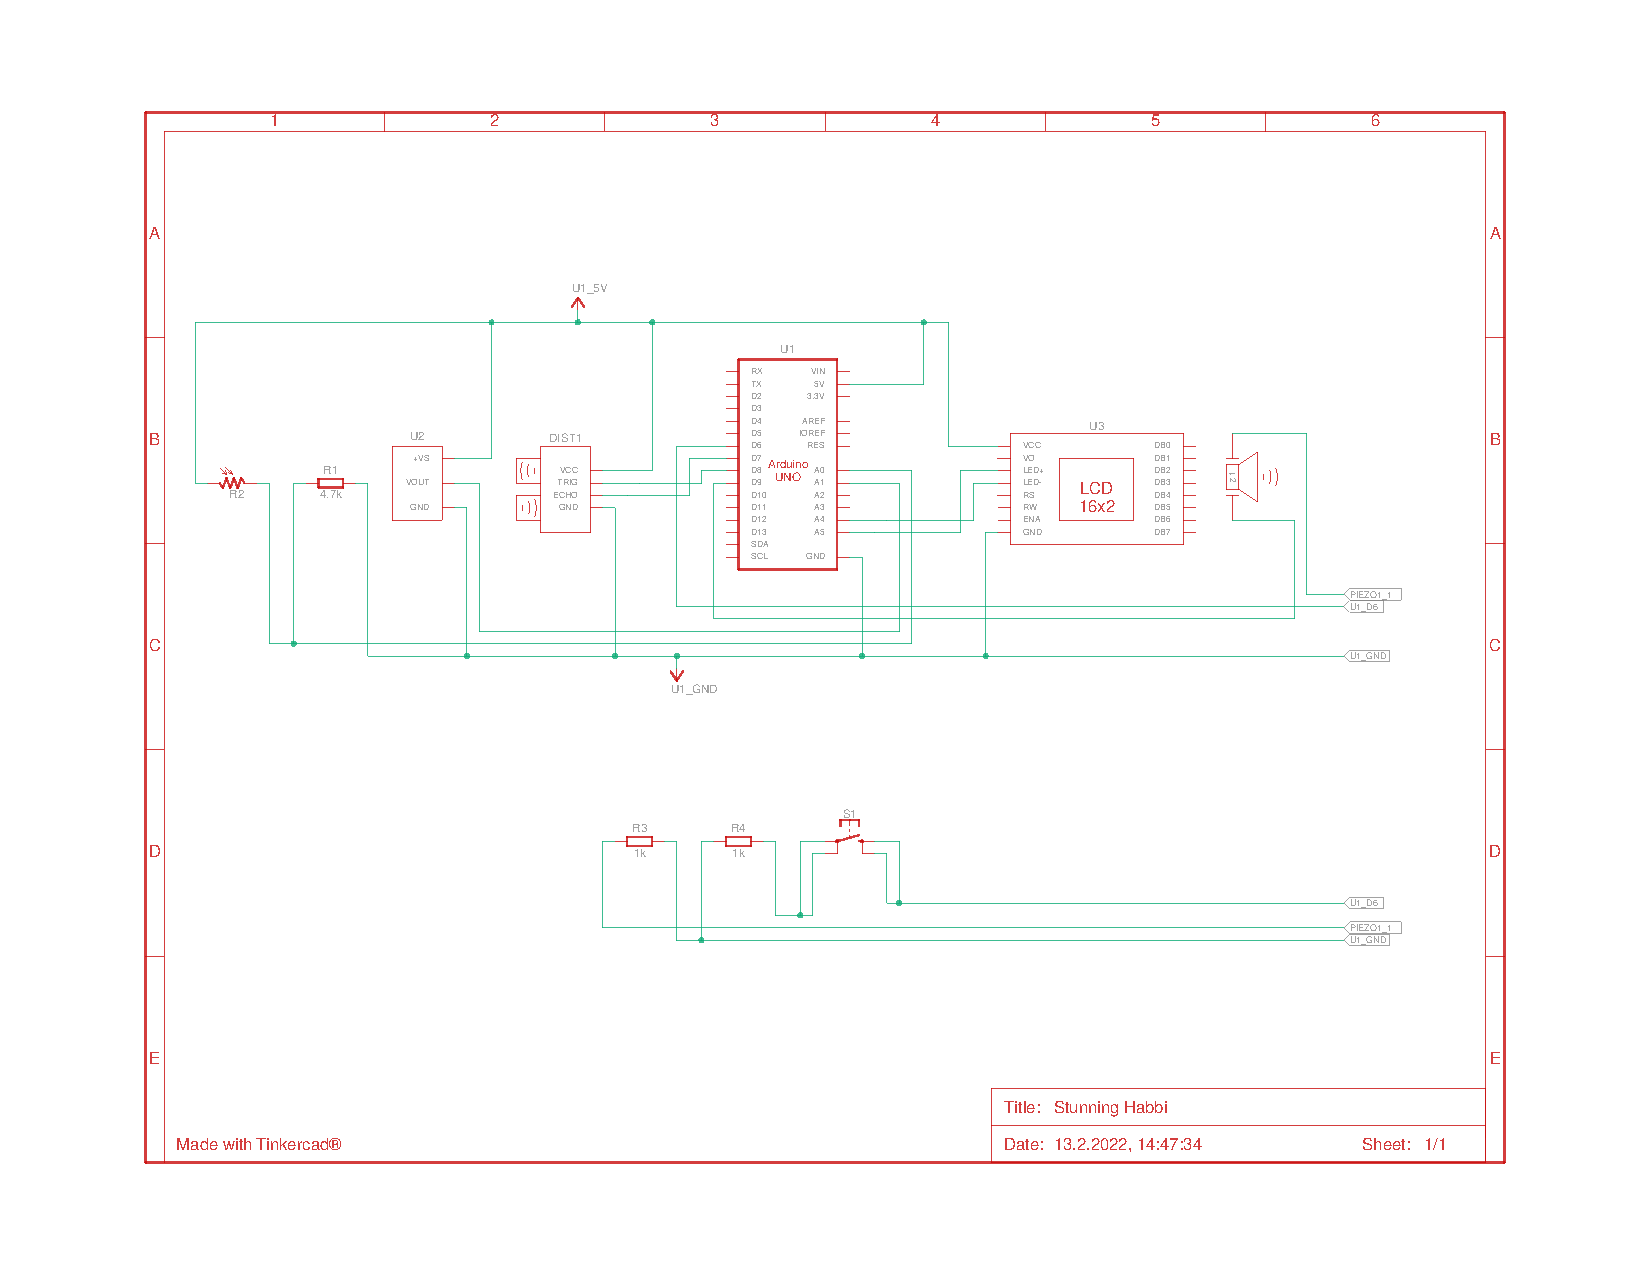
\includegraphics[width=0.45\textwidth, trim={0 2cm 0 2cm}]{images/wiring-diagram.pdf}
    \caption{Wiring Diagram}
    \label{fig:wiring}
    \end {center}
\end{figure}

\begin{figure}[H]%[!ht]
    \begin {center}
    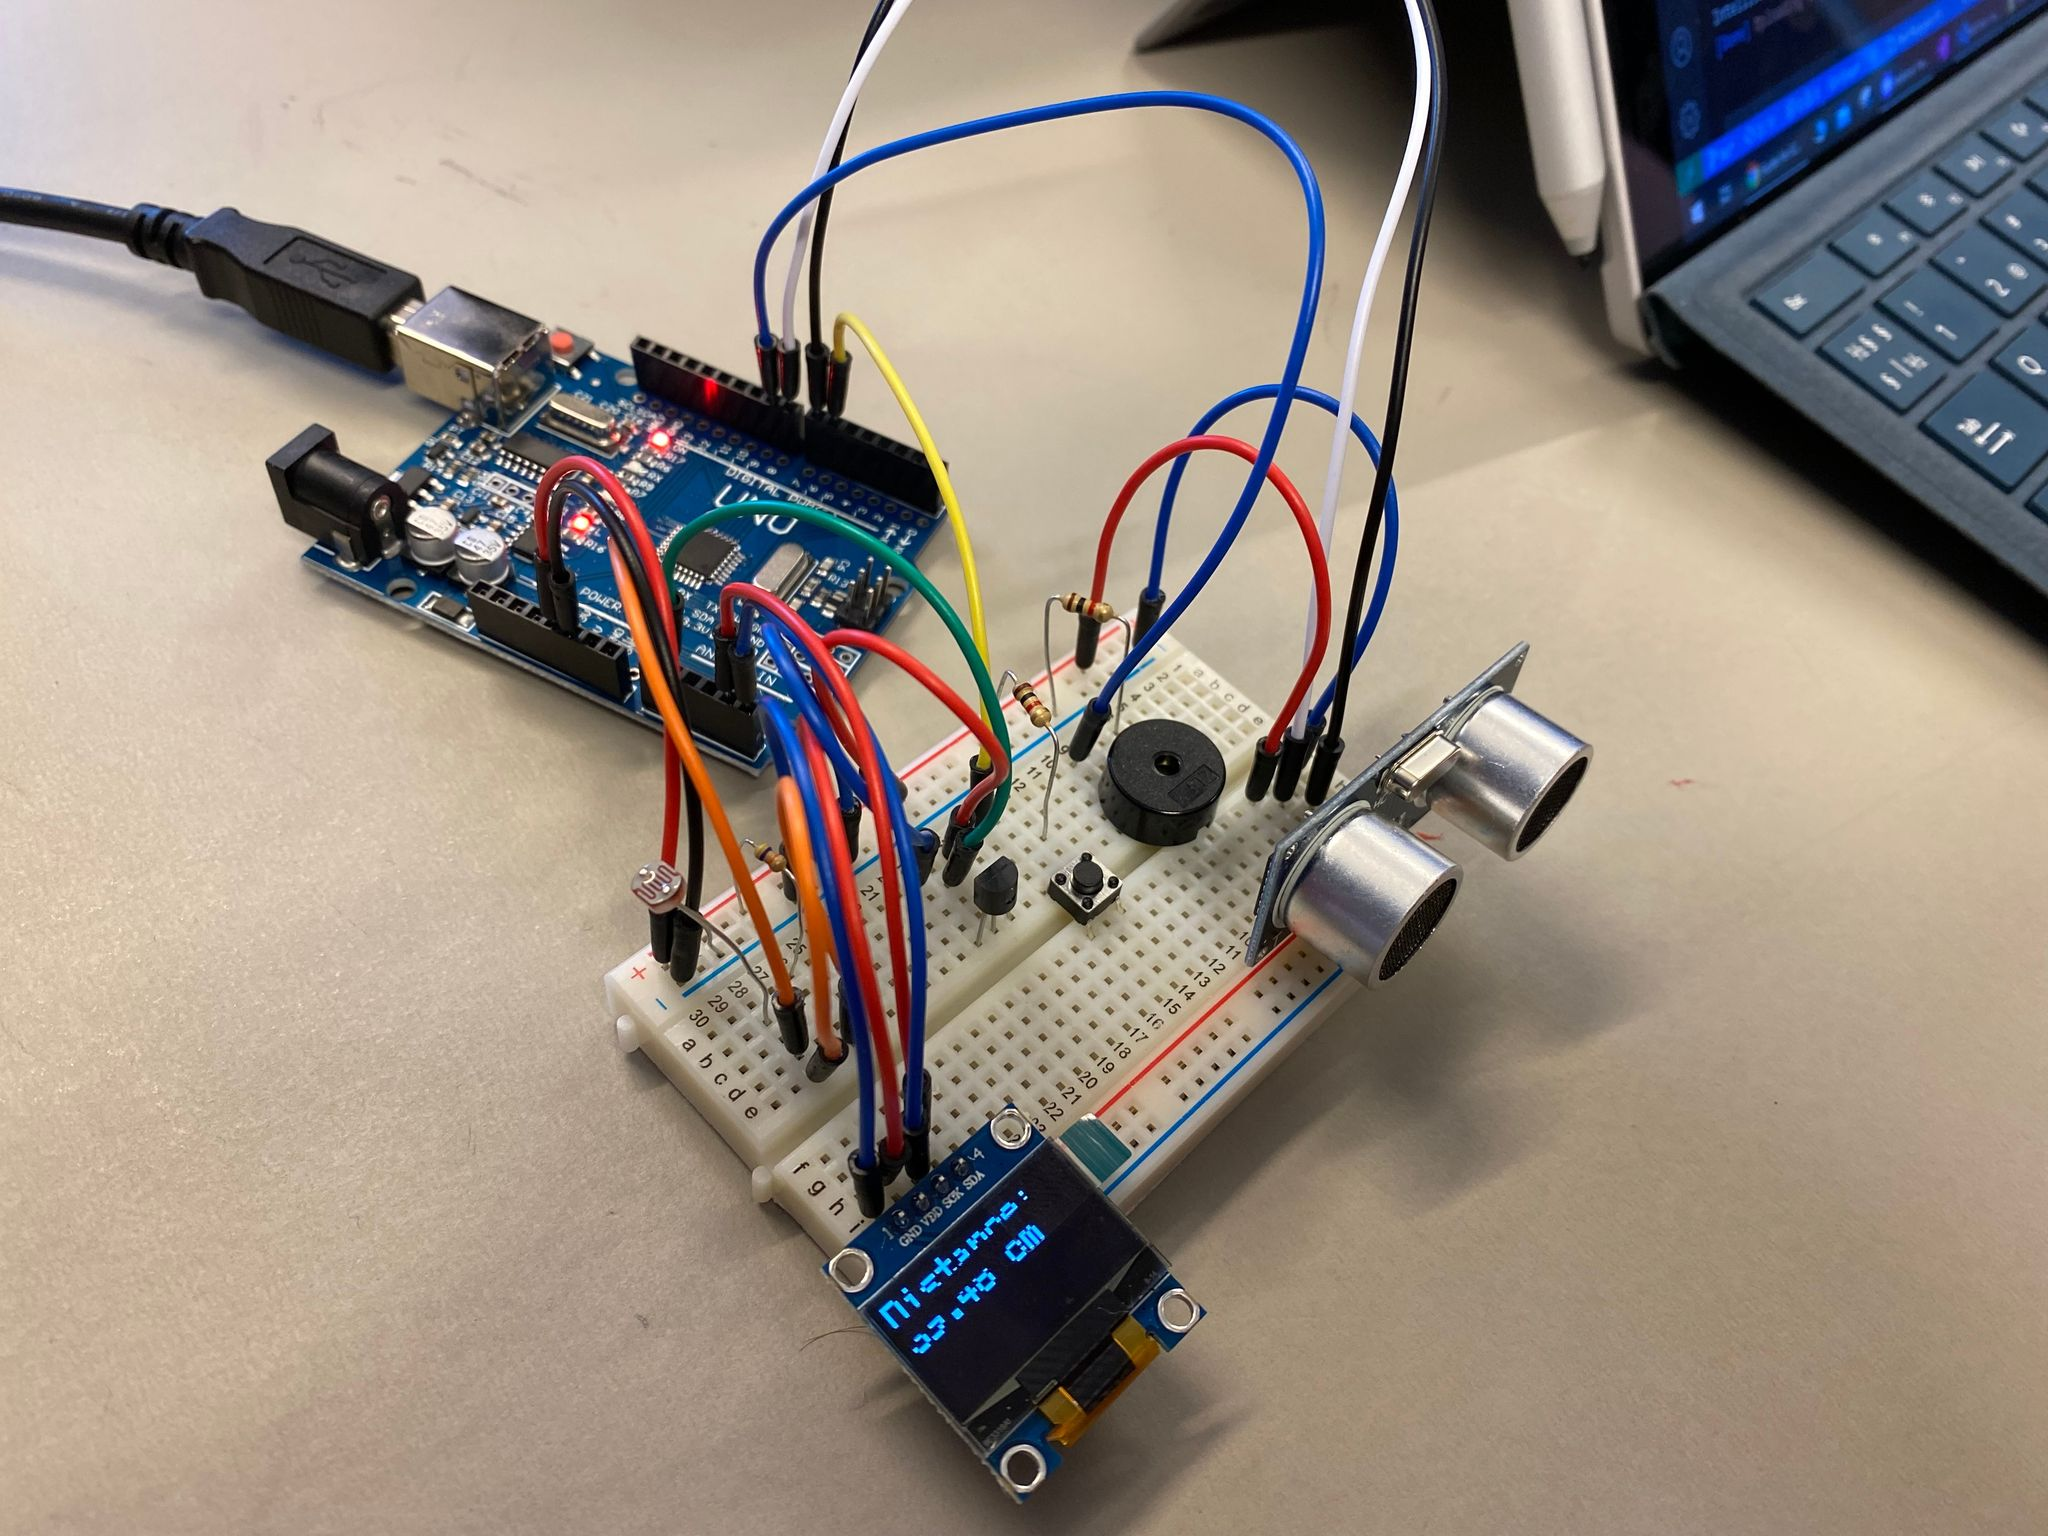
\includegraphics[width=0.45\textwidth]{images/lab1-image.jpg}
    \caption{Lab1 Circuit}
    \label{fig:circuitPicture}
    \end {center}
\end{figure}

\vfill\null
\pagebreak

\subsection{Software}
We start by defining our enums. To keep the code more readable, we split this code into multiple files
\lstinputlisting[language=C++]{../src/AlarmState.h}
For the OledState we also have a function for getting the next OledState value.
This means we also need a header file. This is a language requirement in C++.
\lstinputlisting[language=C++]{../lib/OledState/OledState.h}
In the OledState.cpp file, we can now import the header file and give getNextOledState an implementation.
\lstinputlisting[language=C++]{../lib/OledState/OledState.cpp}
While splitting the code up like this makes for more files and more code to write over all,
it does make for more scalable code. PlatformIO also provides us with a lib folder where we can put such files,
to keep the code more portable,
as well as providing a standardised system for code-splitting.

\vfill\null
\pagebreak

Now that we have defined our external files,
it is time to give the project a configuration.
\lstinputlisting[language=ini]{../platformio.ini}
Under env we specify lib\textunderscore deps which is a list of the Code Libraries this project
uses. This is where PlatformIO shines compared to the ArduinoIDE, as anyone who opens
this project with a PlatformIO compatible IDE (In our case VSCode) will have all dependencies
automatically downloaded with the correct version.\\

We have defined three environments: uno, native and CI. The uno environment
is for compiling the project to the arduino uno. It defines the board and
framework, which is used by PlatformIO behind the scenes to present us with
proper compilation warnings, as well as automatically selecting the
proper procedures for uploading the project.\\

The native environment is intended for testing. Test driven development is a good practice,
and PlatformIO presents us with a solid foundation to do this without needing the
physical board.

\onecolumn

Finally we have the CI environment. CI stands for Continuous Integration,
and refers to a automated build system in github. When code in this project is pushed,
a linux server will automatically run the native tests, and tell the developer if the code
is working and safe to merge into the master branch. This is useful for code developed
in teams, so each team member does not need to run the tests manually to ensure nothing was
broken by their changes. Here is the CI script:
\lstinputlisting[language=yaml, firstline=2]{../../.github/workflows/native_tests.yml}

Now that the CI is set up, lets take a look at our Unit Tests:
\lstinputlisting[language=C++, firstline=2]{../test/test_desktop/OledState/test_OledState.cpp}
The purpose of this code is to check/ASSERT that the code related to the OledState is working properly.
We do this by writing test code that uses the production code, and then checks that
the outputs are what we expect.

Now, lets look at the main.cpp file:
\lstinputlisting[language=C++, firstline=2]{../src/main.cpp}

\begin{multicols}{2}

    By using the median of the last 5 values, we are able to remove high spikes, that would
    cause a large error in the distance measurement. We could use a running-average, however
    such a filter would still have a short-term error. The median filter eliminates
    this issue all together. It is worth noting however, that larger windows in the median filter
    could cause the data to lag behind the real values. In a realtime application, this could
    potentially be unacceptable, and other methods for filtering should be considered.\\

    The code uses the AceButton library to detect button presses. Not only does this lib
    handle debouncing for us, but it also gives us a event based architecture to handle
    clicks. This makes for more readable code.

    \section{Discussion}
    Given my previous experience in the subject, my focus was directed away from
    the circuit and code, and more towards researching best-practices in the IoT industry.
    After many hours, i found PlatformIO, which has presented the most benefits compared
    to the alternatives. With a builtin package manager, as well as its design with modern
    code-practices such as Unit Testing in mind, it stands out as an exceptional tool.
    Furthermore, i took the time to explore more advanced C++ features such as structs,
    allowing me to create a more scalable design for global variables. Currently, all
    configurations such as pins and constants are centralised in the PinConfig and ApplicationConfig.
    This way, the tendency of arduino projects reaching houndreds of globals can be avoided.\\

    I think the way i spent my time on this project prooved productive, and the fruits of may
    labour will likely be reflected in future projects.

    % use section* for acknowledgment
    \section*{Acknowledgment}
    While Kristian Hansen is not a co-author on this paper,
    he did create the circuit diagram in \autoref{fig:wiring},
    while i was working on the code.
    \autoref{fig:circuitPicture}
    is a picture of the circuit used in this project.
    It was created by me and photographed by Kristian.
\end{multicols}

\end{document}


